
\chapter{Model}


\section{Energy Economic model of Europe}
In this section the composition of the energy-economic model used in this project will be described. 

\subsection{Topology}
The model used in  this project is based on the work presented in \cite{PyPSA_euro_30_model}, where a model spanning the electricity grid of 30 European countries is formulated as a techno-economic linear optimization problem. Countries included in the model are the EU-28 countries not including Cyprus and Malta, instead including Norway, Switzerland, Serbia and Bosnia and Herzegovina.

The topology of the network, presented on \ref{fig:network_lay}, is such that each node represents a country and the links represent international HVDC or HVAC links. The links included are based on currently installed international transmission lines. 


\begin{figure}[H]\centering
	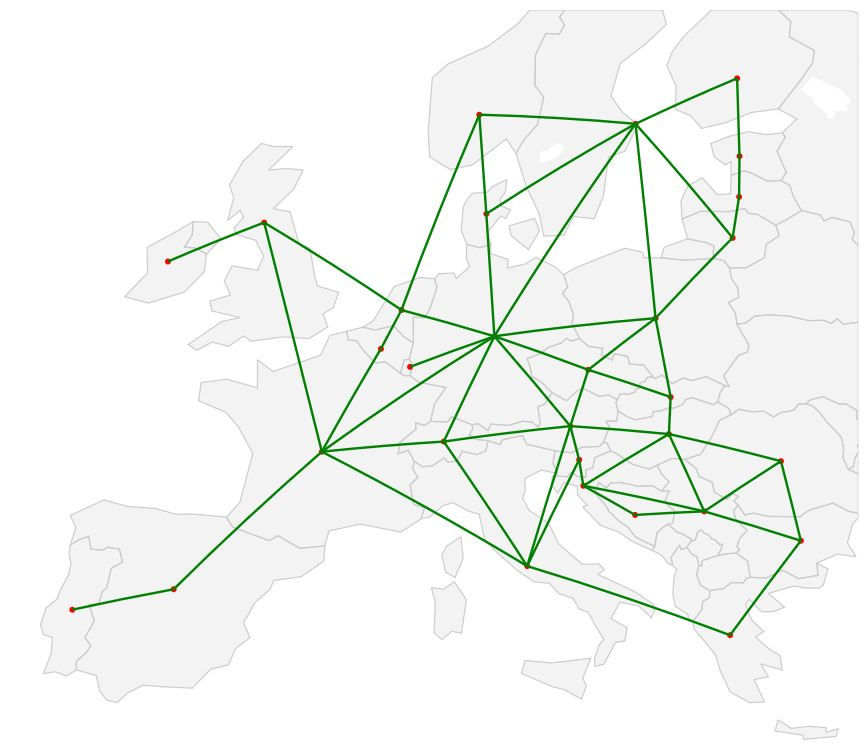
\includegraphics[width=0.75\textwidth]{./Images/network_layout}
	\caption{Network layout}
	\label{fig:network_lay}
\end{figure}


All model input parameters are based on 2011 values as this is the earliest year with all data available. The temporal resolution of the model is hourly, with all simulations spanning a full year. Technology costs are all valued in 2011 Euros. 
Should also be included:
<
\subsection{Energy production}

Each node in the network, has energy producing technologies available, with initial capacities being zero. The available energy producing technologies used in this project is: Onshore wind, offshore wind, Solar PV and OCGT. In the model all technology capacities are expandable limited only be the geographical potential. 

The geographical potentials used are calculated following the work of  \cite{PyPSA_euro_30_model}. In the calculation of geographical potential, the potential available area suited for either onshore wind, offshore wind and solar PV, must first be defined. These areas was found by allowing certain technologies to be installed only in areas with certain land use types. Hereby restricting onshore wind farms from being installed in cities and solar PV plants to be installed in forests etc. The placement of offshore wind farms was restricted to areas with a water depth of less than 50m. Furthermore, all nature reserves was excluded from the potential areas. As competing land use and likely public acceptance issues will occur, the found potential areas are set to bee only 20\% of the found area for onshore and offshore wind and only 1\% for solar PV. 
Assuming a maximum nominal installation density of 10 $MW/km^2$ for offshore and onshore wind power, and 145 $MW/km^2$ for solar PV, it is possible to calculate the geographical potential for the three technologies all across Europe. Geographical potential for the three technologies are presented on figure \ref{fig:geographical_potential}.

\begin{figure}[H]\centering
	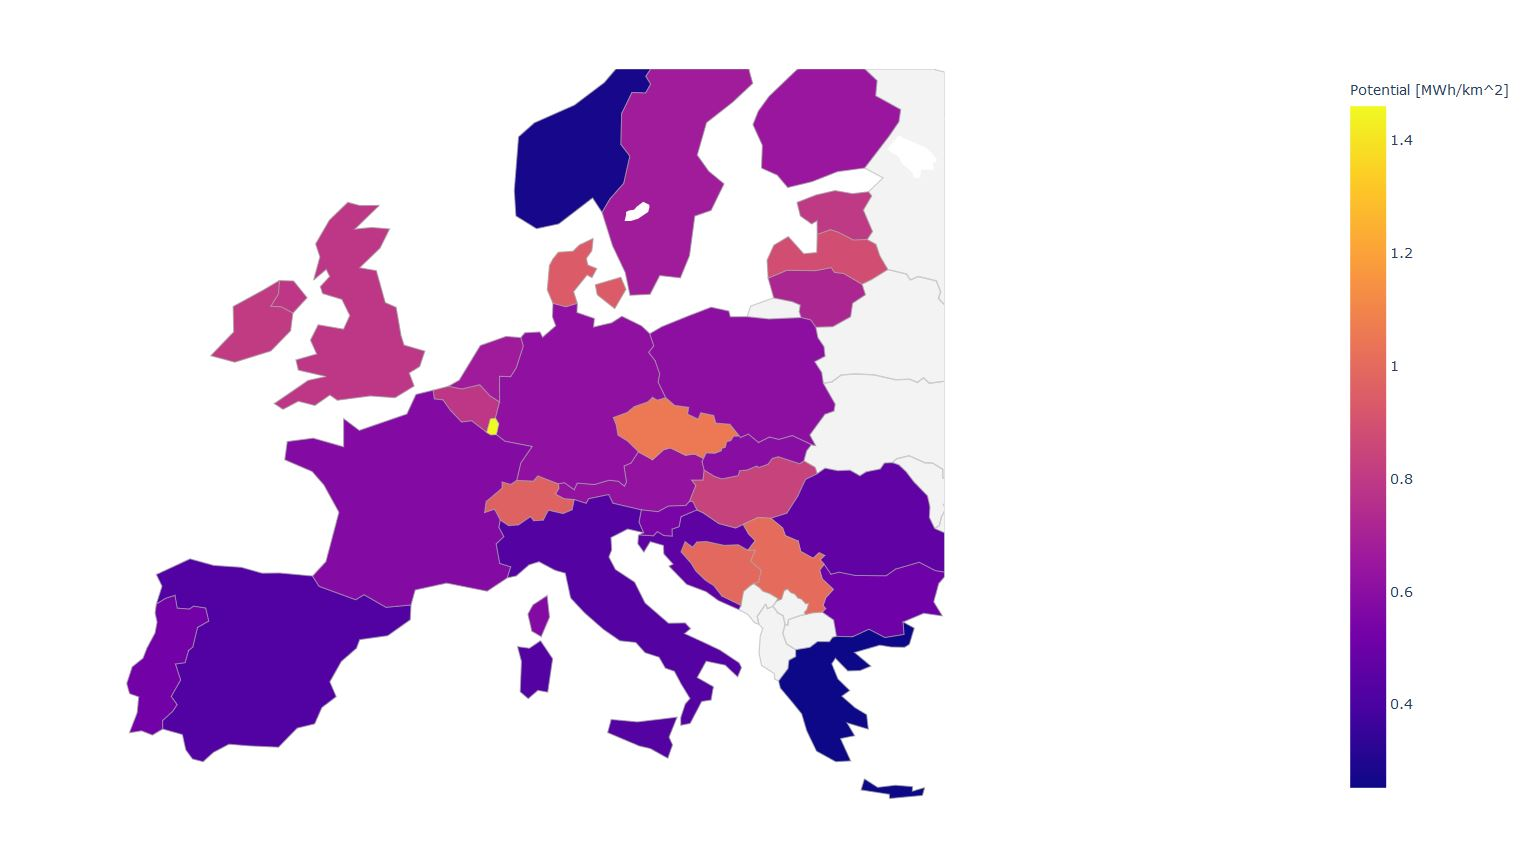
\includegraphics[width=0.95\textwidth]{./Images/geographical_potential}
	\caption{!!! PLACE HOLDER !!! Geographical potential GW/km2}
	\label{fig:geographical_potential}
\end{figure}

The hourly energy production of all variable renewable energy sources is limited by the production potential given by the weather. Following \cite{PyPSA_euro_30_model}, the availability was calculated using historic weather data for 2011 from \cite{ClimateForecastSystem} with a spatial resolution of 40x40 km and hourly temporal resolution. The weather data is first converted to generation potentials for each 40x40 km cell using the REatlas software \cite{ANDRESEN20151074}, and then the national means are found. 


\begin{figure}[H]\centering
	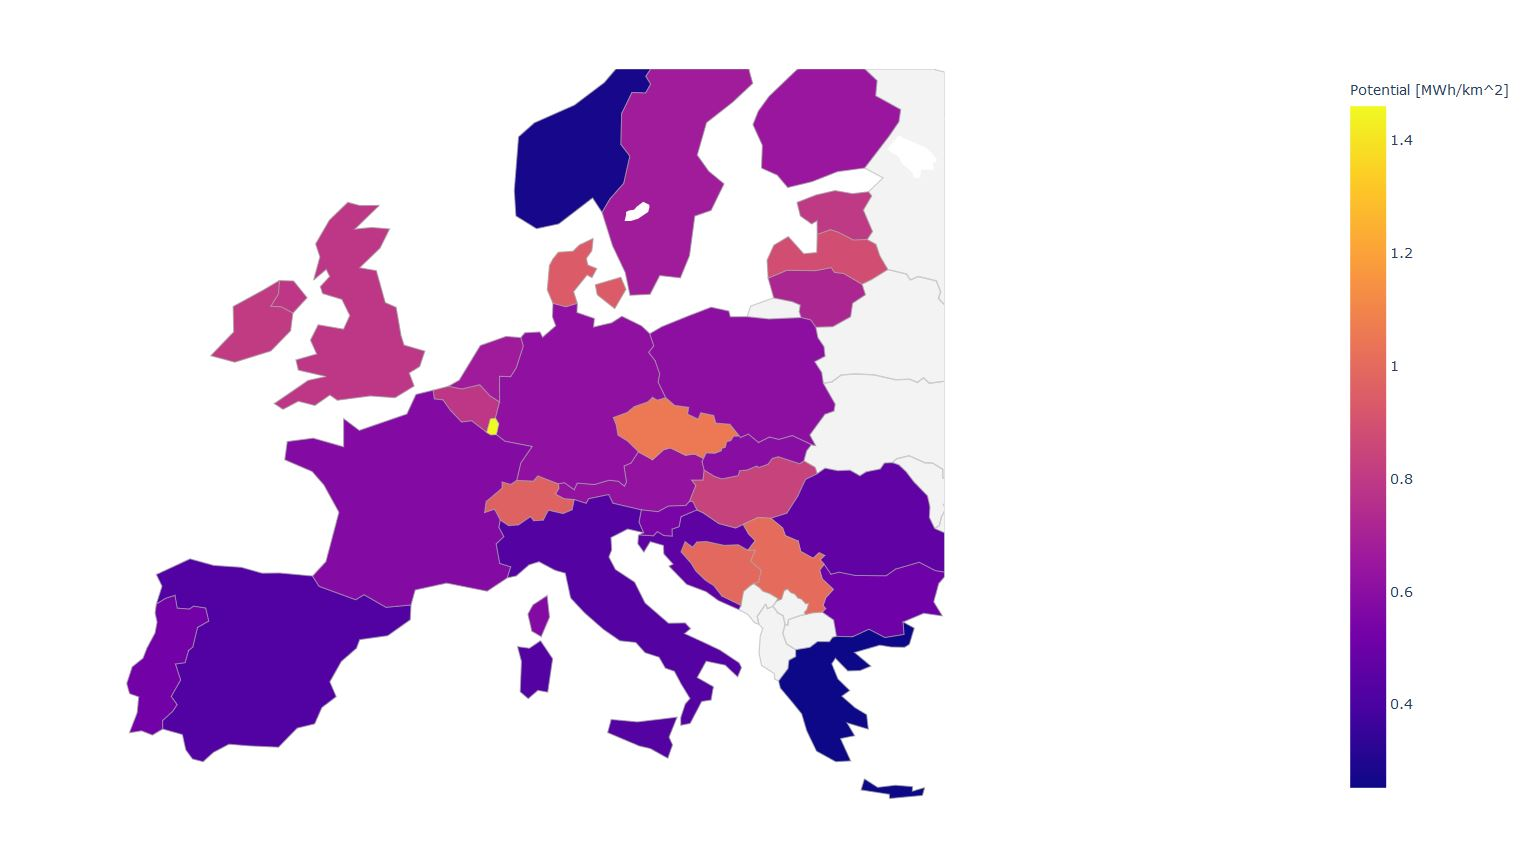
\includegraphics[width=0.95\textwidth]{./Images/geographical_potential}
	\caption{!!! PLACE HOLDER !!! Mean wind generation potential}
	\label{fig:generation_potential}
\end{figure}

The dispatchable energy sources available in all countries are chosen to be open cycle gas turbines (OCGT), as they have a high flexibility and good load following capabilities, therefore making them suitable as a backup generator in a highly decarbonized scenario. They do however not necessarily produce realistic results, when used in scenarios with low decarbonization. The capacities and energy generation of the gas turbines are contrary to the variable renewable energy sources, not limited by geographical or generation potentials. They are however, limited by the maximum allowable CO2 emission. The CO2 emission intensity of the open cycle gas turbine is 0.19 t/MW.


In all simulations the capacities of all energy generators are initially set to be zero, with the capability to be expanded until geographical potentials or CO2 limits further expansion. The cost of expanding capacities is calculated as annualized cost, given as the annualized investment cost plus fixed annual operations and maintenance cost. Annualized investment cost is calculated by multiplying the annuity factor \ref{eq:annuity} by the investment cost. 

\begin{equation}\label{eq:annuity}
a = \frac{r}{1 - \frac{1}{(1+r)^n}}
\end{equation}

Where $r$ is the discount rate, and $n$ is the expected lifetime of the given technology. In this project a discount rate of 7\% is used. The lifetime of the individual technologies are listed in table \ref{tab:cost_data}. All cost data are based on the 2030 values presented in \cite{Schroder2013Current}.

\begin{table}[]
	\begin{tabular}{l|llll}
		Technology      & \makecell[c]{Investement \\ {[}€/MW{]}}	& \makecell[c]{Fixed O\&M \\ {[}€/kW/year{]}} & \makecell[c]{Marginal cost \\ {[}€/MWh{]}}	& \makecell[c]{lifetime \\ {[}years{]}} \\ \hline
		Onshore Wind    &       1182  		&   35      &   0.015       &   25       \\
		Offshore Wind	&		2506		&	80		&	0.02		&	25		\\
		Solar PV   		&       600    		&   25      &   0.01    	&   25       \\
		OCGT       		&       400    		&   15      &   58.4        &   30      \\
		Transmission	& 400 €/MW km +150000 pr line & 2\% & 0 		&   40 
	\end{tabular}
	\caption{Generator parameters are based on the values from \cite{Schroder2013Current}, and transmission parameters are based on the work presented in \cite{HAGSPIEL2014654}.}
	\label{tab:cost_data}
\end{table}

\subsection{Energy demand}
The data for the hourly electricity demand found in the European Network of Transmission System Operators data portal is used as energy demand \cite{ENTSO-E}. The data has a resolution of one hour, and is provided for all countries included in the model. 

\subsection{Energy transmission}
In the model used in this project, all transmission lines are treated as transport models with a coupled source and sink, only constrained by energy conservation at each connecting node. Transmission loss is thereby not considered. This approximation is assumed to be acceptable as most international transmission lines already are, or probably will be in the near future, controllable point-to-point high voltage direct current (HVDC) lines. 

Line capacities initially start as zero, and can then be expanded if found feasible in the optimization, with no constraint on the maximum allowable capacity. The investment cost of line capacity is calculated as a cost pr MWkm plus an additional cost for a high voltage AC to DC converter pair. The price of a high voltage AC to DC converter pair is set to be 150000€ regardless of line capacity \cite{HAGSPIEL2014654}. 

The length of each line is set as the distance between the centroids of each connecting country plus an additional 25\%. The extra 25\% is added to the line length as competitve land use and public acceptance issues will prohibit lines from being placed in optimal positions. 

Furthermore, to satisfy n-1 security the price is adjusted with a factor of $1.5$, to account for the extra installed capacity needed, as shown in \cite{PyPSA_euro_30_model}. 

\begin{equation}
c_l = \left( L*I_s*1.25+150000 \right) *1.5*1.02*a
\end{equation}

1.25 = 25\% extra length due to land use competition
150000 = Price of DC converter pair
1.5 = n-1 security 
1.02 = 2\% FOM (fixed operations and maintanance cost)
a = annuity 




\fxnote{Consider showing some time series for demand etc}







\section{Experiment design}


\subsection{4D experiment}
In this study a four dimensional sub space of the decision space is utilized to explore the characteristics of the model. The four variables in this new space is the total amount of installed gas turbine (ocgt) capacity, wind turbine capacity, solar pv capacity and the total installed transmission capacity. Using a low dimensional space allows for a thorough exploration of the feasible space as the relative fast computation time allows for several studies to be performed using different parameters. 

For every single MGA explorations there are two parameters that can be altered. These are the amount of reduction in CO2 emission compared to the base model, and the amount of MGA slack used. For this experiment it was chosen to iterate over both of these variables exploring CO2 reductions og 0, 50, 80 and 95\%, and MGA slacks of 1, 2, 5, and 10\%. This means that a total of 16 MGA studies is to be performed. 

\subsection{CO2 experiment}

\subsection{Multiplicity experiment}

\subsection{Spatial grouping experiment}


